\section{Preprocessing \& Slice selection}
\nblink{brats/02\_preprocess.ipynb}
\nblink{brats/03\_train\_test\_split.ipynb}

These are also saved as 2 byte integers with the values 0 (not tumor), 1 (todo), 2(todo) and 4(todo).

Every layer is saved as a 2 byte signed integer. We convert these to 1 byte unsigned integers and scale the range to 0-255, so the highest value in the 2 byte signed integer is 255 and the lowest is 0.
This way we generate a grayscale image that can be viewed with a normal image viewer and should be processable by a normal convolutional neural network

\begin{figure}[H]
\centering
\caption{Extracted horizontal slices with merged tumor segment}
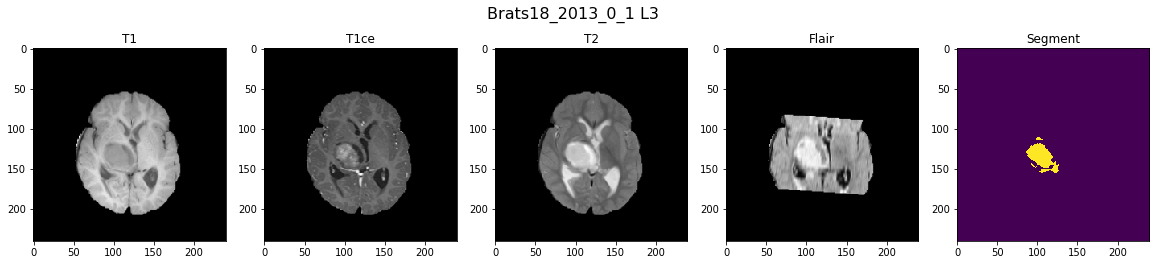
\includegraphics[width=15cm]{chapters/04_segmentation/images/preprocessing.png}
\end{figure}
